\begin{figure}[t]
  \centering
  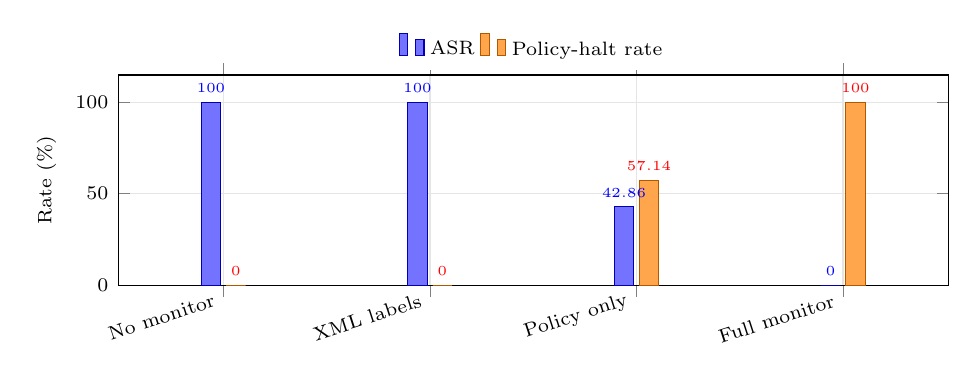
\begin{tikzpicture}
    \begin{axis}[
        width=\columnwidth,
        height=4.25cm,
        ybar,
        bar width=7pt,
        ymin=0,
        ymax=115,
        ylabel={Rate (\%)},
        symbolic x coords={No monitor,XML labels,Policy only,Full monitor},
        xtick=data,
        x tick label style={font=\scriptsize, rotate=18, anchor=east},
        y tick label style={font=\scriptsize},
        ylabel style={font=\scriptsize},
        enlarge x limits=0.17,
        legend style={font=\scriptsize, at={(0.5,1.02)}, anchor=south,
          legend columns=2, draw=none},
        nodes near coords,
        every node near coord/.append style={font=\tiny},
        grid=major,
        grid style={gray!20}
      ]
      \addplot+[fill=blue!55, draw=blue!70!black]
        coordinates {(No monitor,100) (XML labels,100)
          (Policy only,42.86) (Full monitor,0)};
      \addplot+[fill=orange!70, draw=orange!70!black]
        coordinates {(No monitor,0) (XML labels,0)
          (Policy only,57.14) (Full monitor,100)};
      \legend{ASR,Policy-halt rate}
    \end{axis}
  \end{tikzpicture}
  \caption{Controlled ablation outcomes over seven attack paths. Benign
  utility was 100\% for every variant.}
  \label{fig:ablation-results}
\end{figure}
